\documentclass[conference]{IEEEtran}
\IEEEoverridecommandlockouts
% The preceding line is only needed to identify funding in the first footnote. If that is unneeded, please comment it out.
\usepackage{cite}
\usepackage{amsmath,amssymb,amsfonts}
\usepackage{algorithmic}
\usepackage{graphicx}
\usepackage{subcaption}
\usepackage{textcomp}
\usepackage{xcolor}
\usepackage[utf8]{inputenc}
\usepackage[vietnamese]{babel}
\usepackage{amsmath}
\usepackage{float}
\usepackage{natbib}


\def\BibTeX{{\rm B\kern-.05em{\sc i\kern-.025em b}\kern-.08em
    T\kern-.1667em\lower.7ex\hbox{E}\kern-.125emX}}
\usepackage[backend=bibtex,style=ieee]{biblatex}
\addbibresource{ref.bib}

\begin{document}

\title{Forecasting the Vietnam banking’s stock prices using Statistical, Machine Learning and Deep Learning model\\
\thanks{Identify applicable funding agency here. If none, delete this.}
}

\author{\IEEEauthorblockN{1\textsuperscript{st} Tran Ngoc To Nhu}
\IEEEauthorblockA{\textit{Faculty of Information Systems, University of Information Technology} \\
\textit{E-mail: 21520385@gm.uit.edu.vn}}
\and
\IEEEauthorblockN{2\textsuperscript{nd} Le Thuy Duong}
\IEEEauthorblockA{\textit{Faculty of Information Systems, University of Information Technology} \\
\textit{E-mail: 21520203@gm.uit.edu.vn}}
\and
\IEEEauthorblockN{3\textsuperscript{rd} Tran Thanh Huy}
\IEEEauthorblockA{\textit{Faculty of Information Systems, University of Information Technology} \\
\textit{E-mail: 21522170@gm.uit.edu.vn}}
\and
\IEEEauthorblockN{4\textsuperscript{th} Mai Tran Khuong Duy}
\IEEEauthorblockA{\textit{Faculty of Information Systems, University of Information Technology} \\
\textit{E-mail: 21521998@gm.uit.edu.vn}}
\and
\IEEEauthorblockN{5\textsuperscript{th} Vu Tien Linh}
\IEEEauthorblockA{\textit{Faculty of Information Systems, University of Information Technology} \\
\textit{E-mail: 19521760@gm.uit.edu.vn}}
}

\maketitle

\renewcommand{\abstractname}{Abstract}
\begin{abstract}
The integration of information technology into various aspects of life, including economics, healthcare, and commerce, is becoming increasingly prevalent. This trend is particularly evident in areas of heightened interest, where the demand for powerful applications of information technology continues to surge, posing both challenges and opportunities for IT professionals. Amidst this dynamic landscape, stock price prediction for banking institutions has emerged as a topical area of inquiry. This report delves into the prediction of stock prices for three specific banks: MBB, BIDV, and VCB. By employing a diverse array of algorithms encompassing Deep Learning (MICN, LSTM), statistical algorithms (Holt-Winter), and Machine Learning (XGBoost, Linear Regression with CalendarFourier, DeterministicProcess), the study aims to simultaneously predict stock prices and identify the most efficacious algorithm among those considered.
\end{abstract}

\begin{IEEEkeywords}
Stock, Linear Regression, ARIMA, RNN, GRU, LSTM, SARIMAX, Boosting Model, Stacking Model, ResNet, CNN-LSTM
\end{IEEEkeywords}

\section{Introduction}
Time series analysis and forecasting with time stamped values have garnered significant attention in various domains, including energy, climate, and finance.

In the dynamic financial landscape of Vietnam, particularly considering the relatively nascent stock market compared to global counterparts, the recent surge in AI and machine learning has fueled interest among individual investors, institutions, and economists in leveraging these technologies for stock market and stock price prediction.

This research delves into the application of various algorithms, including Holt-Winters, Fully Convolutional Networks (FCN), Multi-Channel Neural Networks (MICN), Extreme Gradient Boosting, and Linear Regression with Calendar Fourier and Deterministic Process, for predicting stock prices in the Vietnamese banking sector. The study also evaluates the performance of these algorithms.

The banking industry plays a pivotal role in steering and supporting the Vietnamese stock market and directly impacts the country's economy. Moreover, it represents a stable sector with significant market capitalization on the Vietnamese stock exchange. Due to the vast number of bank stocks, this study focuses on predicting stock prices for three major banks listed on the Vietnamese stock market.

\section{RELATED WORKS}
Stock market data identification has proven to be a complex task over the years, leading to the development of various time series forecasting methods. As presented in [1], the authors employed a CNN-LSTM model to forecast the stock prices of a company on the stock market based on historical information. The CNN-LSTM model demonstrated high accuracy even when trained on real-time stock market data. By extracting features from stock market data and converting them into tensors (data with more than two dimensions), feature vectors are obtained and fed into the LSTM neural network to identify patterns and subsequently predict stock prices over a specified time horizon.

Poongodi M, Vijayakumar V, and Naveen Chilamkurti gathered publicly available data on the bitcoin blockchain from April 28, 2013, to July 31, 2017, which is available on https://coinmarketcap.com/, and applied the ARIMA model to predict the price of bitcoin.

Previous research has explored different approaches to predict stock prices, which is a difficult task. One study combined two techniques, recurrent neural networks (RNNs) and random forests, and achieved better accuracy in forecasting stock prices.

In their paper, Xiwen Jin and Chaoran Yi conducted a comprehensive evaluation of various machine learning models for stock price prediction. Their findings revealed that LSTM and GRU models outperformed other methods, while Random Forest delivered the least satisfactory results. The R2 scores for the analyzed models were: LSTM (0.84), GRU (0.86), Random Forest Regression (0.51), XGBoost Regression (0.69), Linear Regression (0.73), and LGBM Regression (0.72). These results indicate that XGBoost and Random Forest exhibited inferior performance compared to LSTM and GRU models.

MICN achieves a relative improvement of 17.2% and 21.6% over the multivariate method. It utilizes a combination of CNN and Transformers to effectively utilize the overall information of the input. Firstly, it extracts local features of the data, and then models global correlations on this basis.

Ahmad M. Awajan, Mohd Tahir Ismail, and Sadam Alwadi implemented a hybrid method based on Empirical Mode Decomposition and Holt-Winter (EMD-HW) for stock market forecasting. The stock market data is decomposed by EMD into Intrinsic Mode Functions (IMFs) and residual components. All components are forecasted using the Holt-Winter technique. The forecasted values are then aggregated to obtain the forecasted value for the stock market. The strength of this EMD-HW lies in its ability to forecast non-stationary and nonlinear time series without the need for any transformation methods.

Jizhong Wu, Bo Liu, Hao Zhang, Shumei He, and Qianqian Yang developed a method based on a fully convolutional network (FCN) for fault segmentation and used synthetic seismic data to create an accurate and sufficient training dataset.

\section{MATERIALS}

\subsection{DATASET}
Historical stock prices of 3 banks: Vietnam Joint Stock Commercial Bank for Investment and Development (BIDV), Vietnam Joint Stock Commercial Bank for Foreign Trade (VCB), and Military Commercial Joint Stock Bank (MBB). The data was collected from January 1, 2018, to March 27, 2024. Each dataset contains approximately 1555 rows and includes 7 attributes: Date, Price, Open, High, Low, Vol, Change.

Date: Trading date
Price: Closing price of the stock at the close of trading
Open: Opening price of the stock on the trading day
High: The highest price reached by the stock during the day
Low: The lowest price reached by the stock during the day
Vol: Trading volume of the stock on the day (unit: million shares)
Change: The difference between the closing price and the closing price of the previous day (percentage value)

\subsection{DESCRIPTIVE STATISTICS}
\begin{table}[htbp]
\caption{BIDV, VCB, MBB’s Descriptive Statistics}
\begin{center}
\begin{tabular}{|c|c|c|c|}
\hline
\textbf{} & \textbf{\textit{BIDV}} & \textbf{\textit{VCB}} & \textbf{\textit{MBB}} \\
\hline
Count & 1555 & 1555 & 1555 \\
\hline
Mean & 34182.499 & 69726.468 & 16067.881 \\
\hline
Std & 7693.206 & 16302.756 & 5615.11 \\
\hline
Min & 16531.4 & 35483 & 7206.6 \\
\hline
25\% & 28470.8 & 54907 & 10912.85 \\
\hline
50\% & 33231.4 & 72929 & 15802.5 \\
\hline
75\% & 39924.4 & 81950 & 20493.8 \\
\hline
Max & 54400 & 106500 & 28666.7 \\
\hline
\end{tabular}
\label{tab1}
\end{center}
\end{table}



\begin{minipage}{0.23\textwidth}
    \centering
    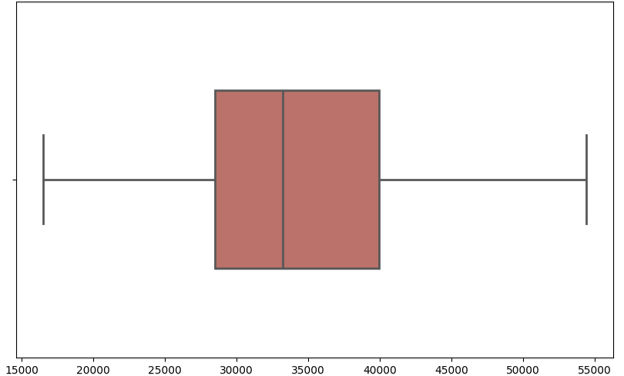
\includegraphics[width=\linewidth]{images/bidv_boxplot.png}
    \captionof{figure}{Box Plot of BIDV stock price (2018 - 2024)}
    \label{fig:image1}
\end{minipage}
\hfill
\begin{minipage}{0.23\textwidth}
    \centering
    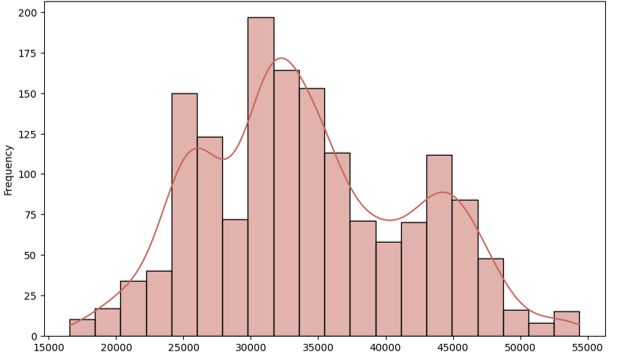
\includegraphics[width=\linewidth]{images/bidv_histogram.png}
    \captionof{figure}{Histogram of BIDV Stock Price (2018 - 2024)}
    \label{fig:image2}
\end{minipage}

\begin{minipage}{0.23\textwidth}
    \centering
    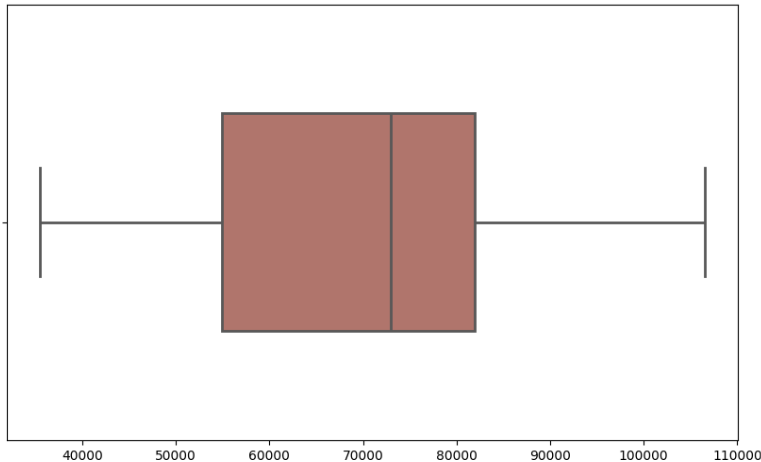
\includegraphics[width=\linewidth]{images/vcb_boxplot.png}
    \captionof{figure}{Box Plot of VCB Stock Price (2018 - 2024)}
    \label{fig:image1}
\end{minipage}
\hfill
\begin{minipage}{0.23\textwidth}
    \centering
    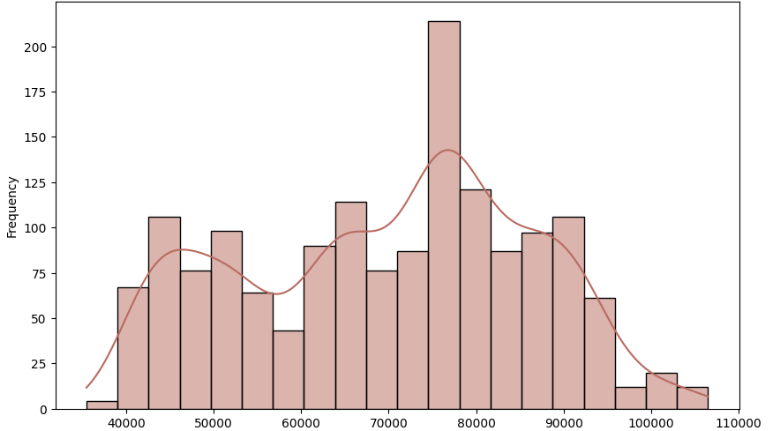
\includegraphics[width=\linewidth]{images/vcb_histogram.png}
    \captionof{figure}{Histogram of VCB Stock Price (2018 - 2024)}
    \label{fig:image2}
\end{minipage}

\begin{minipage}{0.23\textwidth}
    \centering
    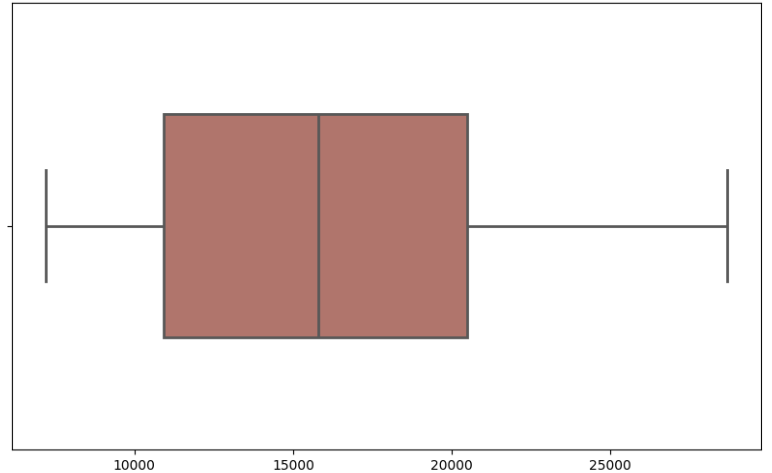
\includegraphics[width=\linewidth]{images/mbb_boxplot.png}
    \captionof{figure}{Box Plot of MB Bank Stock Price (2018 - 2024)}
    \label{fig:image1}
\end{minipage}
\hfill
\begin{minipage}{0.23\textwidth}
    \centering
    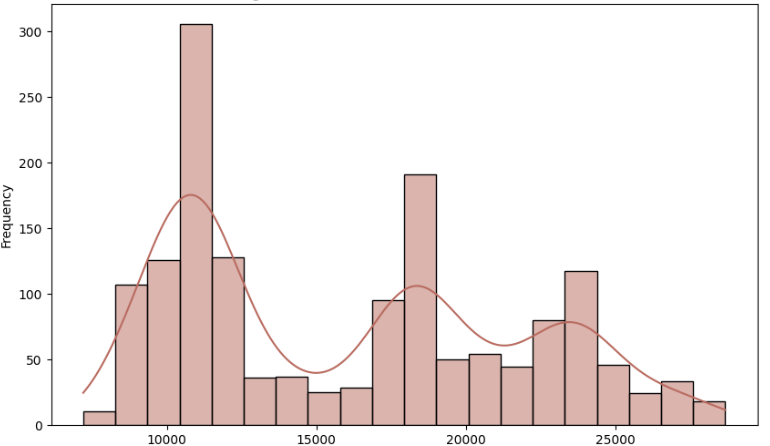
\includegraphics[width=\linewidth]{images/mbb_histogram.png}
    \captionof{figure}{Histogram of MB Bank Stock Price (2018 - 2024)}
    \label{fig:image2}
\end{minipage}


\section{METHODS}
\subsection{ARIMA}

The ARIMA model is a powerful tool for forecasting future values in time series data, particularly when trends and seasonality are present. It leverages past data points (AR term) to understand historical relationships, and corrects for non-stationary behavior (trends or seasonality) by differencing the data a specific number of times (I term). To further refine its predictions, ARIMA incorporates past forecast errors (MA term) to account for any systematic biases. The model is concisely represented as ARIMA(p, d, q), where p signifies the number of past data points included, d indicates the degree of differencing needed for stationarity, and q represents the number of past forecast errors considered.

\[
y_t = \sigma(V_{s_{t}})
\]
Where:
\begin{itemize}
    \item $Y_t$ is the value of the time series at time $t$.
    \item $c$ is a constant term.
    \item $\phi_1, \phi_2, \ldots, \phi_p$ are the autoregressive parameters.
    \item $\theta_1, \theta_2, \ldots, \theta_q$ are the moving average parameters.
    \item $e_t$ is the error term at time $t$.
    \item $p$ and $q$ are the orders of the autoregressive and moving average components, respectively.
\end{itemize}




\subsection{Linear Regression}
Linear regression is a statistical method for modeling the relationship between a dependent variable and one or more independent variables. It assumes a linear relationship and aims to find the best-fit line that minimizes the difference between predicted and actual values. It's used to predict outcomes and understand the impact of variables in fields like economics, finance, and machine learning.

A Linear regression model that includes 2 regression, and a single independent variable is called simple regression and a regression model that involves two or more independent variables is called multiple regression. Simple linear regression is just a special case of multiple linear regression. A multiple linear regression model has the form: \cite{linearRegressionMethod} \\
\[Y=\beta_0+\beta_1X_1+\beta_2X_2+\cdots+\beta_kX_k+\varepsilon\]
Where:\\
	\indent\textbullet\ Y is the dependent variable (Target Variable).\\
	\indent\textbullet\ \(X_1, X_2, \ldots, X_k\) are the independent (explanatory) variables.\\
	\indent\textbullet\ \(\beta_0\) is the intercept term.\\
	\indent\textbullet\ \(\beta_1,..., \beta_k\) are the regression coefficients for the independent variables.\\
	\indent\textbullet\ \(\varepsilon\) is the error term.

\subsection{Holt Winter}
The Holt Winters (HW) method is an extension of the Holt method, and is applied whenever the data behaviour is trendy and is seasonal. Relatively to the seasonal type, it can be additive or multiplicative, depending on the oscillatory movement along the time period. In both versions, forecasts will depend on the following three components of a seasonal time series: its level, its trend and its seasonal coefficient. \cite{HoltWinter1} Exponential smoothing is a technique used to smooth out a time series data by assigning decreasing weights exponentially to past observations, thereby reducing the influence of older data points on the overall smoothed result.
There are three main variants of Exponential Smoothing: Single Exponential Smoothing, Double Exponential Smoothing, and Triple Exponential Smoothing.
The specific formula for Single Exponential Smoothing is: \cite{HoltWinter2}
\begin{align*}
S_t = \alpha \cdot y_t + (1 - \alpha) \cdot (S_{t-1} + b_{t-1}) 0 < α < 1
\\
b_t = \gamma \cdot (S_t - S_{t-1}) + (1 - \gamma) \cdot b_{t-1} 0 < γ < 1 
\end{align*}
Where: 
\begin{itemize}
\item $b_t$ is the smoothed estimate of the average growth at the end of period $t$.
\item $\gamma$ is the smoothing parameter for the trend, typically ranging from $0$ to $1$.
\item $b_{t-1}$ is the previous smoothed estimate of the trend at the end of period $t-1$.
\item $S_t$ is the smoothed estimate of the level at the end of period $t$.
\item $S_{t-1}$ is the smoothed estimate of the level at the end of period $t-1$.
\end{itemize}

Triple Exponential Smoothing extends Double Exponential Smoothing by including a seasonal component to handle time series with seasonality. The specific formula for Triple Exponential Smoothing is: \cite{HoltWinter3}
\begin{align*}
    S_t = \alpha \frac{y_t}{I_{t-L}} + (1-\alpha)(S_{t-1}+b_{t-1}) 
\end{align*}

Where:
\begin{itemize}
\item $S_t$ represents the smoothed observation at time $t$.
\item $y_t$ is the actual observation at time $t$.
\item $I_{t-L}$ is the seasonal index for the same season in the previous year.
\item $\alpha$ is a constant that needs to be estimated.
\item $b_t$ represents the trend factor at time $t$.
\end{itemize}
\begin{align*}
b_t = \gamma (S_t - S_{t-1}) + (1 - \gamma)b_{t-1} & &
\end{align*}

Where:
\begin{itemize}
\item $(b_t)$ captures the trend component.
\item $(\gamma)$ is another constant to be estimated.
\end{itemize}
\begin{align*}
 I_t = \beta \frac{y_t}{S_t} + (1 - \beta) I_{t-L} & &
\end{align*}

Where:
\begin{itemize}
\item $(I_t)$ represents the seasonal index at time $(t)$.
\item $(\beta)$ is yet another constant to estimate.
\end{itemize}
\begin{align*}
F_{t+m} = (S_t + m b_t) I_{t-L+m} & &
\end{align*}

Where:
\begin{itemize}
\item $(F_{t+m})$ is the forecast at $(m)$ periods ahead.
\item $(m)$ represents the number of periods into the future.
\end{itemize}


\subsection{Linear Regression (Calendar Fourier, Deterministic Process)}
Linear Regression Calendar Fourier is a method that transforms temporal data into Fourier frequency components to handle cyclical elements in the data. This can be useful in identifying yearly, monthly, weekly, etc. factors in the data. This method is used to model periodic cycles and variations in temporal data. The basic idea of Fourier regression is to use sine and cosine wave functions to represent a periodic function. In the case of linear regression, we will use these wave functions as independent variables in the linear regression model. \cite{FourierTimeSeries}

\[Y = \beta_0 + \beta_1 \cos(\omega t) + \beta_2 \sin(\omega t) + \ldots + \beta_n \cos(k \omega t) + \beta_{n+1} \sin(k \omega t)\]

Where:
\begin{itemize}
    \item \(\omega = \frac{2\pi}{T}\) is the angular frequency, where \(T\) represents the period.
    \item \(k\) is the number of repetitions in the Fourier series.
\end{itemize}

Linear Regression applied Deterministic Process is a method for modeling deterministic factors in time series data. It assumes that data follows a defined process and models it based on predefined functions. These functions can be linear or nonlinear functions, and they can represent temporal factors such as trends, seasons, cycles, etc.

\[Y = \beta_0 + B_1 X_1 t + \beta_2 X_2 t + \beta_n X_n t\]

Where:
\begin{itemize}
    \item \(Y\) is the dependent variable.
    \item \(\beta_0\) is the intercept or constant term.
    \item \(B_1, \beta_2, \ldots, \beta_n\) are the coefficients associated with the corresponding independent variables \(X_1, X_2, \ldots, X_n\).
    \item \(t\) is the independent variable.
\end{itemize}

\subsection{XGBoost}
XGBoost(eXtreme Gradient Boosting) is a machine learning model based on Gradient Boosting but optimized and processed in parallel to significantly improve model training time.\\
XGBoost performs a simple search of many different decision trees and then uses the decision tree results and previous error levels as input for the next decision tree search step. After a certain number of iterations or acceptance threshold, stop the algorithm. \cite{XGBoost}\\
XGBoost algorithm work:
\begin{itemize}
    \item Consider a function or estimate . To start, we build a sequence derived from the function gradients. The equation below models a particular form of gradient descent. The represents the Loss function to minimize hence it gives the direction in which the function decreases. is the rate of change fitted to the loss function, it’s equivalent to the learning rate in gradient descent. is expected to approximate the behaviour of the loss suitably.
    \[F_{x_{t+1}} = F_{x_t} + \epsilon_{x_t} \frac{\partial F}{\partial x}(x_t)\]
    \item To iterate over the model and find the optimal definition we need to express the whole formula as a sequence and find an effective function that will converge to the minimum of the function. This function will serve as an error measure to help us decrease the loss and keep the performance over time. The sequence converges to the minimum of the function . This particular notation defines the error function that applies when evaluating a gradient boosting regressor.
    \[f(x, \theta) = \sum l(F((X_i, \theta), y_i))\]
\end{itemize}


\subsection{RNN}
An RNN is a neural network that combines variable-length input data with a hidden state that depends on previous time steps to produce output data. Through the connections among hidden units associated with the time delay, the model can retain information about the past, enabling it to discover temporal correlations between events that are far away from each other in the data. \cite{RNN}\\
The standard model of RNN is illustrated as the picture below: \\

\begin{figure}[H]
    \centering
    \begin{minipage}{0.8\linewidth}
    \centering
        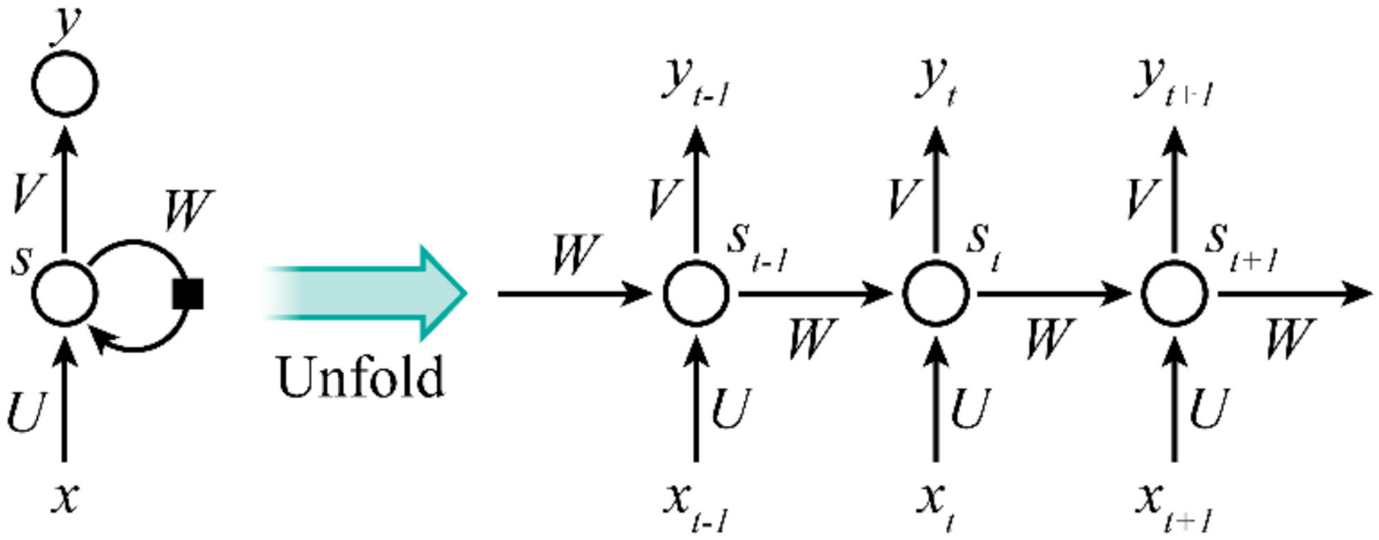
\includegraphics[width=\linewidth]{images/RNNModel.png}
    \caption{Standard RNN model (Source: \cite{DeepLearning})}
    \label{fig7}
    \end{minipage}
\end{figure}
The hidden state \( S_t \) at step \( t \) is calculated based on the input \( X_t \) at step \( t \) and the hidden state \( S_{t-1} \) from the previous step:
\[
s_{t} = f(U_{x_{t}} + W_{s_{t-1}})
\]
Where:
\begin{itemize}
    \item \( s_t \): Hidden state at time \( t \).
    \item \( x_{t} \): Input at time \( t \).
    \item \( s_{t-1} \): Hidden state at time \( t-1 \).
    \item \( U \): Weight matrix from the input to the hidden state.
    \item \( W \): Weight matrix from the previous hidden state to the current hidden state.
    \item \( f \): Activation function (commonly the tanh or sigmoid function).
\end{itemize}

\[
y_t = \sigma(V_{s_{t}})
\]

Where:
\begin{itemize}
    \item \( y_t \): Output at time \( t \).
    \item \( s_{t} \): Hidden state at time \( t \).
    \item \( V \): Weight matrix from the hidden state to the output.
    \item \( sigma \): Activation function. 
\end{itemize}

\subsection{GRU}
Kyunghyun Cho was the first to introduce GRU in 2014. It is an RNN-based algorithm that is comparableto LSTM but has a simpler architecture. The fundamental problem of RNN is the vanishing and explodinggradient issue, which occurs due to continuous multiplication during Backpropagation Through Time. GRU addresses this problem by using gates, namely the update gate and reset gate.\cite{ComparisonGRU&ARIMA}
\begin{figure}[H]
    \centering
    \begin{minipage}{0.8\linewidth}
    \centering
        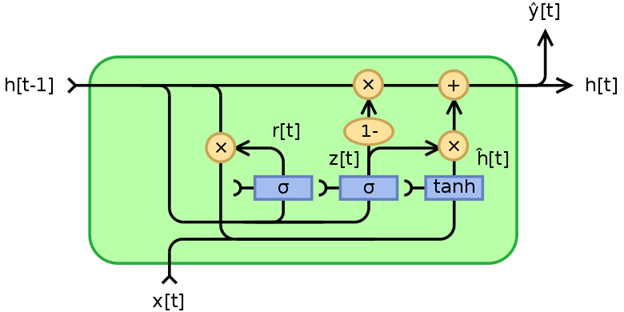
\includegraphics[width=\linewidth]{images/GRU.png}
    \caption{The architecture of the GRU model}
    \label{fig8}
    \end{minipage}
\end{figure}
GRU Architecture:
Reset gate: defines how much past information must be preserved.
\[r_t = \sigma(W_r x_t + [h_{t-1}, x_t] + b_r)\]
Update gate: defines how much of the prior information should be deleted and how to combine the incoming input with the old information.
\[z_t = \sigma(W_z x_t + [h_{t-1}, x_t] + b_z)\]
Candidate hidden state: that will be used by the reset gate to retain important information from the past
\[\tilde{h}_t = \tanh(W_h [r_t \odot h_{t-1}, x_t] + b_h)\]
Hidden state: serves as the output.
\[h_t = (1 - z_t) * h_{t-1} + z_t * \tilde{h}_t\]
Where:
\begin{itemize}
    \item $W_r, W_z, W_h$ are weights matrices.
    \item $x_t$ is the input at time step $t$.
    \item $h_{t-1}$ is the previous hidden state.
    \item $h_t$ is the current hidden state.
    \item $\tilde{h}_t$ is the candidate hidden state.
\end{itemize}


\subsection{LSTM}
LSTM (Long short-term memory) is a type of recurrent neural network (RNN) that was introduced by Hochreiter and Schmid Huber in 1997. It was designed to overcome the limitations of traditional RNN models in capturing and remembering long-term dependencies in sequential data. \cite{LSTM}

\begin{figure}[H]
    \centering
    \begin{minipage}{0.8\linewidth}
    \centering
        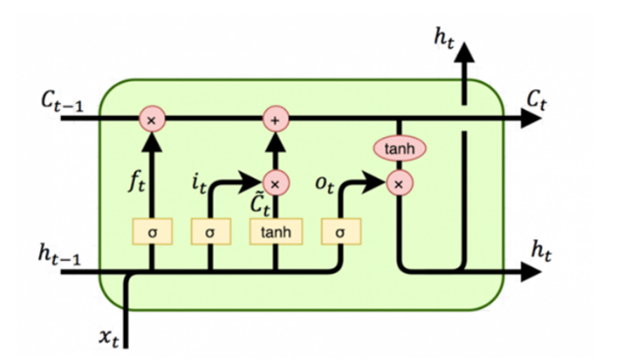
\includegraphics[width=\linewidth]{images/LSTM.png}
    \caption{The architecture of the LSTM model}
    \label{fig9}
    \end{minipage}
\end{figure}
In this model,
\begin{itemize}
    \item $\sigma(z)$ is the sigmoid function:
    \[\sigma = \frac{1}{1 + e^{-x}}\]
    \item tanh is the tanh activation function:
    \[\tanh(x) = \frac{e^x - e^{-x}}{e^x + e^{-x}}\]
\end{itemize}
In state t:
\begin{itemize}
    \item $c_{t-1}$, $h_{t-1}$, $x_t$ : are the output of the previous layer
    \item Output: $c_t$,$h_t$: c is cell state, h is hidden state
\end{itemize}
Gate mechanisms:
\begin{itemize}
    \item Forgot gate: $f_t = \sigma(U_f \cdot x_t + W_t \cdot h_{t-1} + b_f)$
    \item Input gate: $i_t = \sigma(U_i \cdot x_t + W_i \cdot h_{t-1} + b_i)$
    \item Output gate: $o_t = \sigma(U_o \cdot x_t + W_o \cdot h_{t-1} + b_o)$
\end{itemize}
In these formular: W and U refer to the weight matrices used in the computations of the LSTM cell. $b_f$ , $b_i$, $b_o$ are bias for the respective gates.
The equations for the cell state, candidate cell state and the final ouput:
\[\tilde{C}_t = \tanh(W_c \cdot x_t + U_c \cdot h_{t-1} + b_c)\]
\[C_t = f_t \cdot C_{t-1} + i_t \cdot \tilde{C}_t\]
\[h_t = o_t \cdot \tanh(C_t)\]

\subsection{CNN-LSTM}
CNN-LSTM (Convolutional Neural Network - Long Short-Term Memory) combines two important neural network architectures in the field of image and sequence data processing.
As the name implies, CNN-LSTM consists of 2 parts: CNN and LSTM. Specifically, CNN helps in tracking the features of dataset and LSTM helps in tracking the patterns, allowing to train on them \cite{PredictStockCNNLSTM}. \\
\subsubsection{Convolutional Neural Network (CNN):}
\begin{itemize}
    \item CNNs are mainly used in image processing, but can also be applied to other data sequences such as text.
    \item CNN has the ability to learn local features of data by applying filters (kernels) that slide across the input data space.
    \item Convolutional and Pooling layers in CNN help reduce data dimensionality and create characteristic representations of input data.
\end{itemize}

\subsubsection{Long Short-Term Memory (LSTM):}
\begin{itemize}
    \item LSTM is a type of recurrent neural network (RNN) designed to process and understand sequence data with variable length.
    \item The LSTM has three states that help the network to reduce the long term dependency of the data. These states are called the Forget State, the Input State and the Output State \cite{ComparasionCNNLSTM}.
    \item LSTM is widely used in long-term prediction algorithms and natural language processing.
\end{itemize}

\subsubsection{CNN-LSTM architecture:}
\begin{figure}[H]
    \centering
    \begin{minipage}{0.8\linewidth}
    \centering
        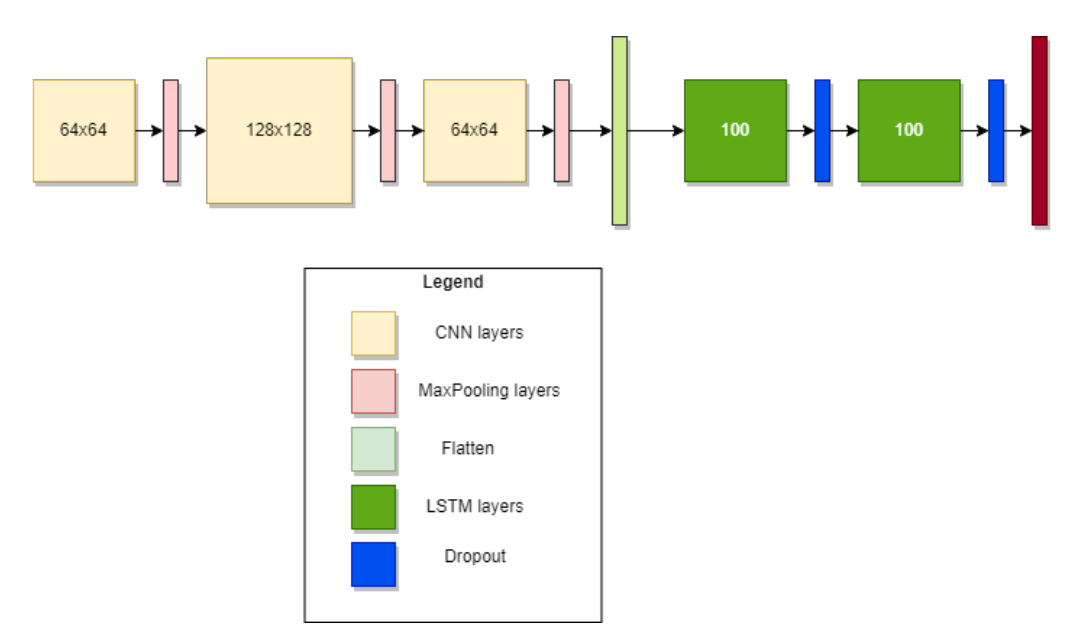
\includegraphics[width=\linewidth]{images/CNNLSTM_Architechture.png}
    \caption{The architecture of the CNN-LSTM model}
    \label{fig10}
    \end{minipage}
\end{figure}

The CNN-LSTM architecture involves using Convolutional Neural Network (CNN) layers for feature extraction on input data combined with LSTMs to support sequence prediction \cite{PredictStockCNNLSTM}.


\subsection{MICN}
The overall structure of MICN is shown in Figure 1. The long time series prediction task is to predict a future series of length O based on a past series of length I, which can be expressed as input (I), predict (O), where O is much larger than I. Inspired by traditional time series decomposition algorithms. We design a multi-scale hybrid decomposition (MHDecomp) block to separate complex patterns of input series. Then we use Seasonal Prediction Block to predict seasonal information and Trend-cyclical Prediction Block to predict trend-cyclical information. Then add the prediction results up to get the final prediction Ypred . We donate d as the number of variables in multivariate time series and D as the hidden state of the series. \cite{MICN}

\begin{figure}[H]
    \centering
    \begin{minipage}{0.8\linewidth}
    \centering
        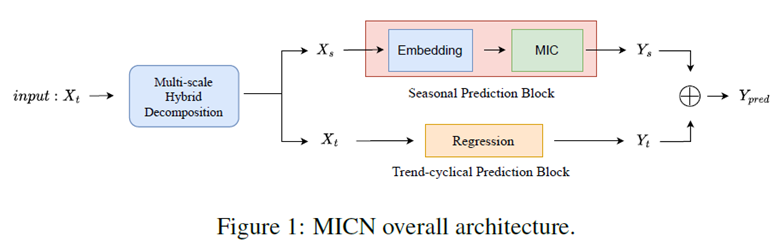
\includegraphics[width=\linewidth]{images/MICN.png}
    \caption{The architecture of the GRU model}
    \label{fig11}
    \end{minipage}
\end{figure}

\subsubsection{MULTI-SCALE HYBRID DECOMPOSITION}
Previous series decomposition algorithms (Wu et al., 2021b) adopt the moving average to smooth out periodic fluctuations and highlight the long-term trends. For the input series \(X \in \mathbb{R}^{I \times d}\), the process is:
\[X_t = \text{AvgPool}(\text{Padding}(X))_{\text{kernel}}\]
\[X_5 = X - X_t\]
where: \(X_t\), \(X_s \in \mathbb{R}^{I \times d}\) denote the trend-cyclical and seasonal parts, respectively.

We use simple mean operation to integrate these different patterns because we cannot determine the weight of each pattern before learning its features. Correspondingly, we put this weighting operation in the Merge part of Seasonal Prediction block after the representation of the features. Concretely, for the input series \(X \in \mathbb{R}^{I \times d}\), the process is:

\[X_t = \text{mean}(\text{AvgPool}(\text{Padding}(X))_{\text{kernel}_1}, \ldots, \text{AvgPool}(\text{Padding}(X))_{\text{kernel}_n})\]
\[X_5 = X - X_t\]
where: \(X_t, X_s \in \mathbb{R}^{I \times d}\) denote the trend-cyclical and seasonal parts, respectively.

\subsubsection{TREND-CYCLICAL PREDICTION BLOCK}
Use a simple linear regression strategy to make a prediction about the trend-cyclical series \(X_t \in \mathbb{R}^{I \times d}\), demonstrating that simple modeling of trend-cyclical is also necessary for non-stationary series forecasting tasks. For the trend-cyclical series \(X_t\) obtained with the MHDecomp block, the process is:
\[Y{\substack{\text{regre}\\t}}{} = regression(X_t)\]
where \(Y_{\text{regre}t} \in \mathbb{R}^{O \times d}\) denotes the prediction of the trend part using the linear regression strategy. And use MICN-regre to represent the MICN model with this trend-cyclical prediction method.

\subsubsection{SEASONAL PREDICTION BLOCK}
After embedding the input sequence Xs, they adopt multi-scale isometric convolution to capture the local features and global correlations, and branches of different scales model different underlying patterns of the time series. They then merge the results from different branches to complete comprehensive information utilization of the sequence. It can be summarised as follows:
\[X{\substack{\text{emb}\\s}}{} = {\text{Embedding}}(\text{Concat}(X_s, X_{\text{zero}}))\]
\[Y{\substack{\text{0}\\s}}{} = X{\substack{\text{emb}\\s}}{}\]
\[Y_{s,l} = \text{MIC}(Y_{s,l-1}), \quad l \in \{1, 2, \ldots, N\}\]
\[Y_s = \text{Truncate}(\text{Projection}(Y_{s,N}))\]

Where:
\begin{itemize}
    \item \(X_{\text{zero}} \in \mathbb{R}^{O \times d}\) denotes the placeholders filled with zeros
    \item \(X_{\text{emb}}^s \in \mathbb{R}^{(I+O) \times D}\) denotes the embedded representation of \(X_s\)
    \item \(Y_{s,l} \in \mathbb{R}^{(I+O) \times D}\) represents the output of the \(l\)-th multi-scale isometric convolution (MIC) layer
    \item \(Y_s \in \mathbb{R}^{O \times d}\) represents the final prediction of the seasonal part after a linear function projection with \(Y_{s,N} \in \mathbb{R}^{(I+O) \times D}\) and a truncate operation.
\end{itemize}

\section{RESULT}

\subsection{EVALUATION METHODS}
The Mean Percentage Absolute Error (MAPE) is a metric used to evaluate the accuracy of a forecasting model. It measures the average absolute percentage difference between the predicted values and the actual values. 
\[\text{MAPE} = \frac{1}{n} \sum_{t=1}^{n} \left| \frac{y_i - \hat{y}_i}{y_i} \right| \times 100\%\]

Root Mean Squared Error (RMSE): measures the average deviation of the predicted values from the actual values, considering the square of the errors. Lower RMSE values indicate better model performance, with zero indicating perfect predictions.
\[\text{RMSE} = \sqrt{\frac{1}{n} \sum_{i=1}^{n} (y_i - \hat{y}_i)^2}\]

Mean Absolute Error (MAE): measure the average absolute difference between the predicted values and the actual values. It provides a straightforward assessment of the model's accuracy, where lower values indicate better performance.
\[\text{MAE} = \frac{1}{n} \sum_{i=1}^{n} |y_i - \hat{y}_i|\]

Where:
\begin{itemize}
    \item \(n\): Number of observations
    \item \(y_i\): Actual value of dependent variable for observation \(i\)
    \item \(\hat{y}_i\): Predicted value of dependent variable for observation \(i\)
\end{itemize}


\subsection{EVALUATION}

\begin{table}[h]
\centering
\caption{BIDV DATASET’S EVALUATION}
\begin{tabular}{lcccc}
\toprule
\textbf{Model} & \textbf{Ratio} & \textbf{RMSE} & \textbf{MAE} & \textbf{MAPE (\%)} \\ \midrule
\multirow{3}{*}{Linear} & 7:3 & 4163.263 & 3495.94 & 8.636 \\
                        & 8:2 & 5320.862 & 4595.571 & 9.835 \\
                        & \textbf{9:1} & \textbf{4152.676} & \textbf{3433.859} & \textbf{7.263} \\ \midrule
\multirow{3}{*}{ARIMA} & 7:3 & 9678.42 & 8347.492 & 18.688 \\
                        & 8:2 & 7109.504 & 6341.757 & 13.607 \\
                        & \textbf{9:1} & \textbf{4192.145} & \textbf{3547.97} & \textbf{7.89} \\ \midrule
\multirow{3}{*}{XGBoost} & 7:3 & 1792.35 & 1154.98 & 2.64 \\
                        & 8:2 & 2027.27 & 1255.36 & 2.63 \\
                        & \textbf{9:1} & \textbf{2301.83} & \textbf{1519.39} & \textbf{3.14} \\ \midrule
\multirow{3}{*}{GRU} & 7:3 & 0.172 & 0.0199 & 20.053 \\
                        & 8:2 & 0.133 & 0.016 & 13.828 \\
                        & \textbf{9:1} & \textbf{0.108} & \textbf{0.02} & \textbf{9.992} \\ \midrule
\multirow{3}{*}{RNN} & 7:3 & 0.169 & 0.0198 & 19.707 \\
                        & 8:2 & 0.131 & 0.019 & 13.529 \\
                        & \textbf{9:1} & \textbf{0.106} & \textbf{0.018} & \textbf{9.899} \\ \midrule
\multirow{3}{*}{LSTM} & 7:3 & 0.175 & 0.029 & 20.213 \\
                        & 8:2 & 0.135 & 0.02 & 14.252 \\
                        & \textbf{9:1} & \textbf{0.106} & \textbf{0.019} & \textbf{9.917} \\ \midrule
\multirow{3}{*}{CNN-LSTM} & 7:3 & 0.17 & 0.03 & 19.741 \\
                        & 8:2 & 0.146 & 0.069 & 14.719 \\
                        & \textbf{9:1} & \textbf{0.101} & \textbf{0.027} & \textbf{9.474} \\ \bottomrule
\end{tabular}
\end{table}

\begin{table}[h]
\centering
\caption{VCB DATASET’S EVALUATION}
\begin{tabular}{lcccc}
\toprule
\textbf{Model} & \textbf{Ratio} & \textbf{RMSE} & \textbf{MAE} & \textbf{MAPE (\%)} \\ \midrule
\multirow{3}{*}{Linear} & 7:3 & 10516.514 & 9124.137 & 11.16 \\
                        & 8:2 & 6513.819 & 5312.01 & 5.823 \\
                        & \textbf{9:1} & \textbf{7900.247} & \textbf{7158.703} & \textbf{8.26} \\ \midrule
\multirow{3}{*}{ARIMA} & 7:3 & 13425.949 & 11325.76 & 12.562 \\
                        & 8:2 & 13349.47 & 12204.32 & 13.159 \\
                        & \textbf{9:1} & \textbf{3863.947} & \textbf{3021.476} & \textbf{3.374} \\ \midrule
\multirow{3}{*}{XGBoost} & 7:3 & 3466.83 & 2066.86 & 2.26 \\
                        & 8:2 & 4145.83 & 2638.60 & 2.77 \\
                        & \textbf{9:1} & \textbf{1426.46} & \textbf{1097.16} & \textbf{1.23} \\ \midrule
\multirow{3}{*}{RNN} & 7:3 & 0.156 & 0.021 & 17.172 \\
                        & 8:2 & 0.113 & 0.0197 & 11.126 \\
                        & \textbf{9:1} & \textbf{0.064} & \textbf{0.019} & \textbf{6.397} \\ \midrule
\multirow{3}{*}{LSTM} & 7:3 & 0.156 & 0.024 & 17.225 \\
                        & 8:2 & 0.118 & 0.02 & 11.898 \\
                        & \textbf{9:1} & \textbf{0.064} & \textbf{0.016} & \textbf{6.578} \\ \midrule
\multirow{3}{*}{CNN-LSTM} & 7:3 & 0.157 & 0.035 & 17.251 \\
                        & 8:2 & 0.104 & 0.036 & 10.197 \\
                        & \textbf{9:1} & \textbf{0.059} & \textbf{0.021} & \textbf{6.119} \\ \bottomrule
\end{tabular}
\end{table}

\begin{table}[h]
\centering
\caption{MBB DATASET’S EVALUATION}
\begin{tabular}{lcccc}
\toprule
\textbf{Model} & \textbf{Ratio} & \textbf{RMSE} & \textbf{MAE} & \textbf{MAPE (\%)} \\ \midrule
\multirow{3}{*}{Linear} & 7:3 & 6699.874 & 6089.079 & 32.65 \\
                        & 8:2 & 5730.287 & 5514.895 & 29.412 \\
                        & \textbf{9:1} & \textbf{4114.666} & \textbf{3621.554} & \textbf{19.495} \\ \midrule
\multirow{3}{*}{ARIMA} & 7:3 & 2958.645 & 2641.558 & 14.258 \\
                        & 8:2 & 2476.036 & 1614.404 & 7.586 \\
                        & \textbf{9:1} & \textbf{2647.877} & \textbf{1890.612} & \textbf{8.649} \\ \midrule
\multirow{3}{*}{XGBoost} & 7:3 & 626.85 & 493.50 & 2.61 \\
                        & 8:2 & 425.11 & 305.03 & 1.57 \\
                        & \textbf{9:1} & \textbf{429.89} & \textbf{316.95} & \textbf{1.55} \\ \midrule
\multirow{3}{*}{RNN} & 7:3 & 0.125 & 0.017 & 16.234 \\
                        & 8:2 & 0.136 & 0.014 & 16.99 \\
                        & \textbf{9:1} & \textbf{0.094} & \textbf{0.015} & \textbf{10.521} \\ \midrule
\multirow{3}{*}{LSTM} & 7:3 & 0.129 & 0.02 & 16.865 \\
                        & 8:2 & 0.137 & 0.014 & 17.237 \\
                        & \textbf{9:1} & \textbf{0.096} & \textbf{0.015} & \textbf{10.714} \\ \midrule
\multirow{3}{*}{CNN-LSTM} & 7:3 & 0.153 & 0.104 & 25.773 \\
                        & 8:2 & 0.133 & 0.023 & 16.963 \\
                        & \textbf{9:1} & \textbf{0.105} & \textbf{0.028} & \textbf{11.551} \\ \bottomrule
\end{tabular}
\end{table}

\subsection{VISUALIZATION}

\subsubsection{BIDV DATASET VISUALIZATION}

\begin{minipage}{0.23\textwidth}
    \centering
    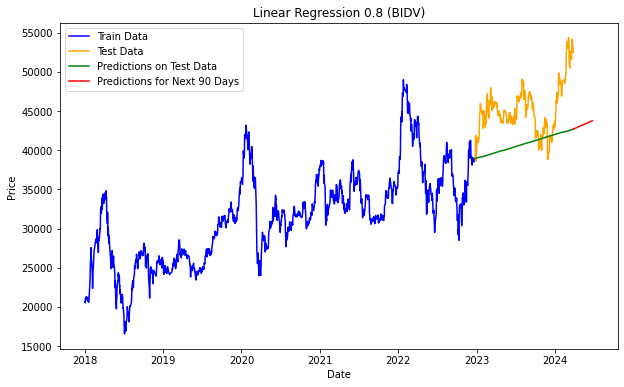
\includegraphics[width=\linewidth]{images/LR/LinearRegression_BIDV_90days_82.png}
    \captionof{figure}{Linear Regression with 8:2 ratio}
    \label{fig:image1}
\end{minipage}
\hfill
\begin{minipage}{0.23\textwidth}
    \centering
    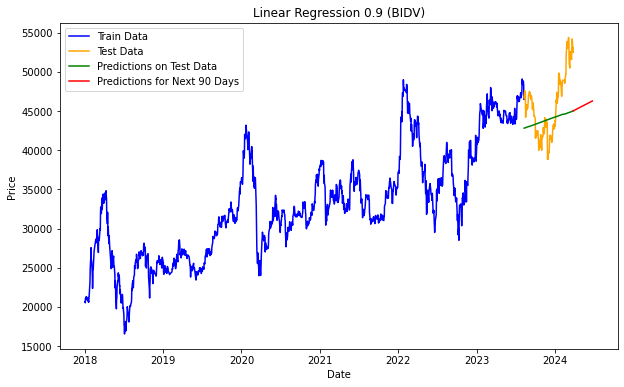
\includegraphics[width=\linewidth]{images/LR/LinearRegression_BIDV_90days_91.png}
    \captionof{figure}{Linear Regression with 9:1 ratio}
    \label{fig:image2}
\end{minipage}

\begin{minipage}{0.23\textwidth}
    \centering
    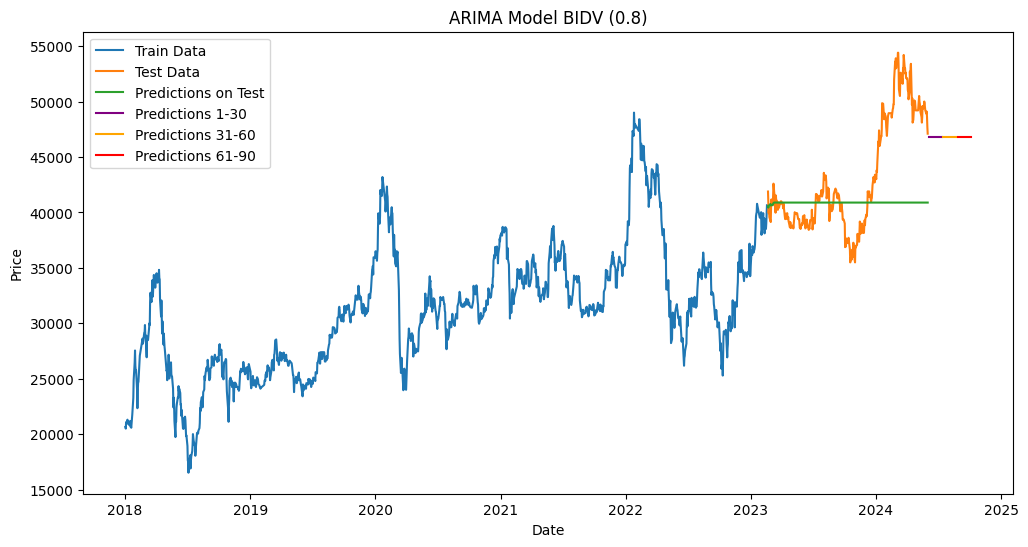
\includegraphics[width=\linewidth]{images/ARIMA/ARIMA_BIDV_82.png}
    \captionof{figure}{ARIMA with 8:2 ratio}
    \label{fig:image1}
\end{minipage}
\hfill
\begin{minipage}{0.23\textwidth}
    \centering
    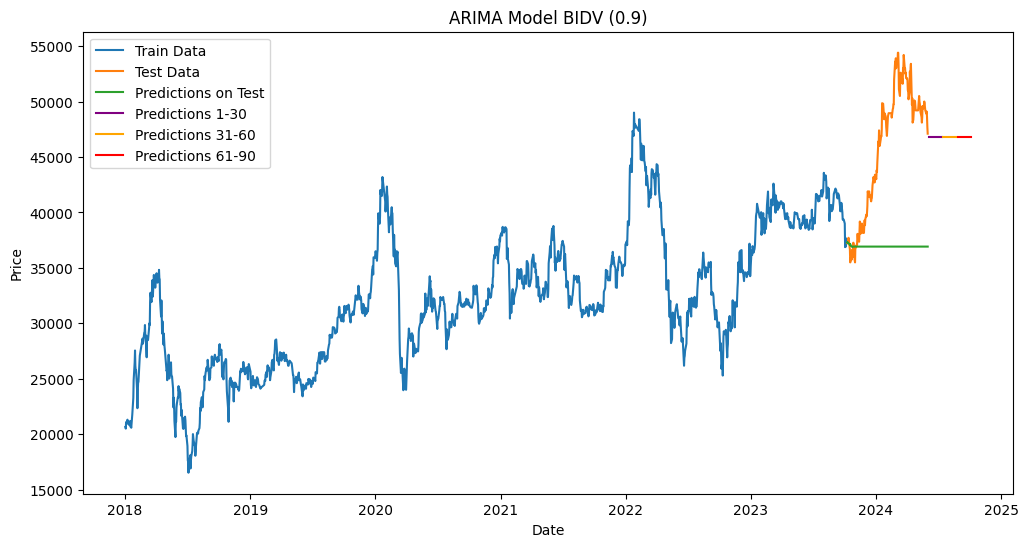
\includegraphics[width=\linewidth]{images/ARIMA/ARIMA_BIDV_91.png}
    \captionof{figure}{ARIMA with 9:1 ratio}
    \label{fig:image2}
\end{minipage}

\begin{minipage}{0.23\textwidth}
    \centering
    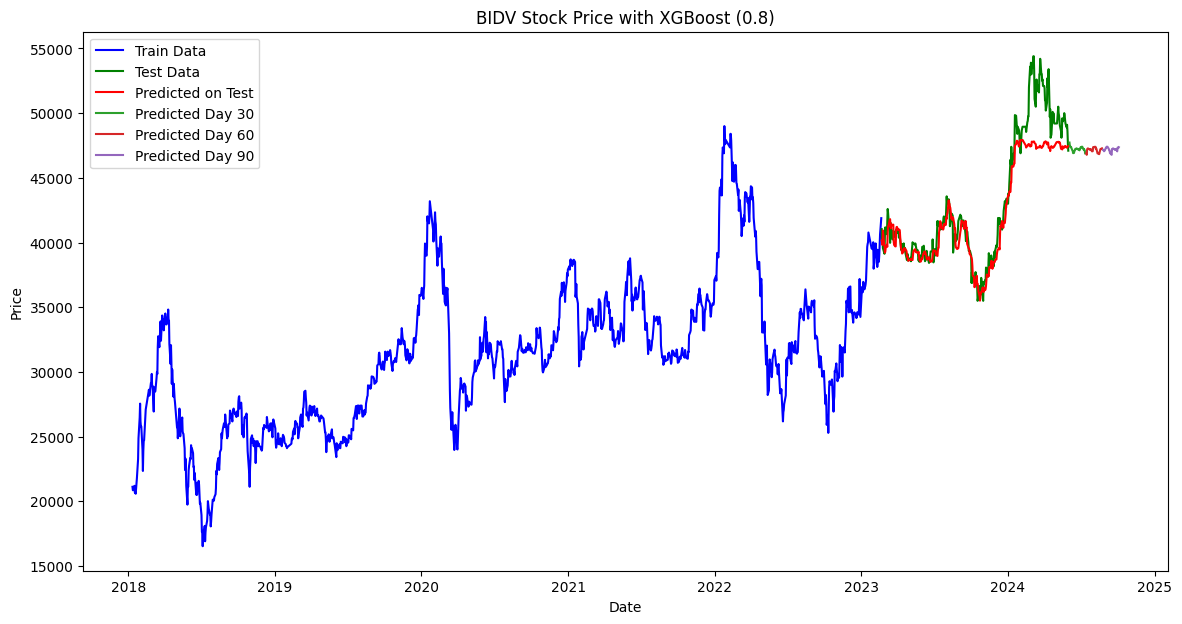
\includegraphics[width=\linewidth]{images/XGBoost/XGBoost_BIDV_82.png}
    \captionof{figure}{XGBoost with 8:2 ratio}
    \label{fig:image1}
\end{minipage}
\hfill
\begin{minipage}{0.23\textwidth}
    \centering
    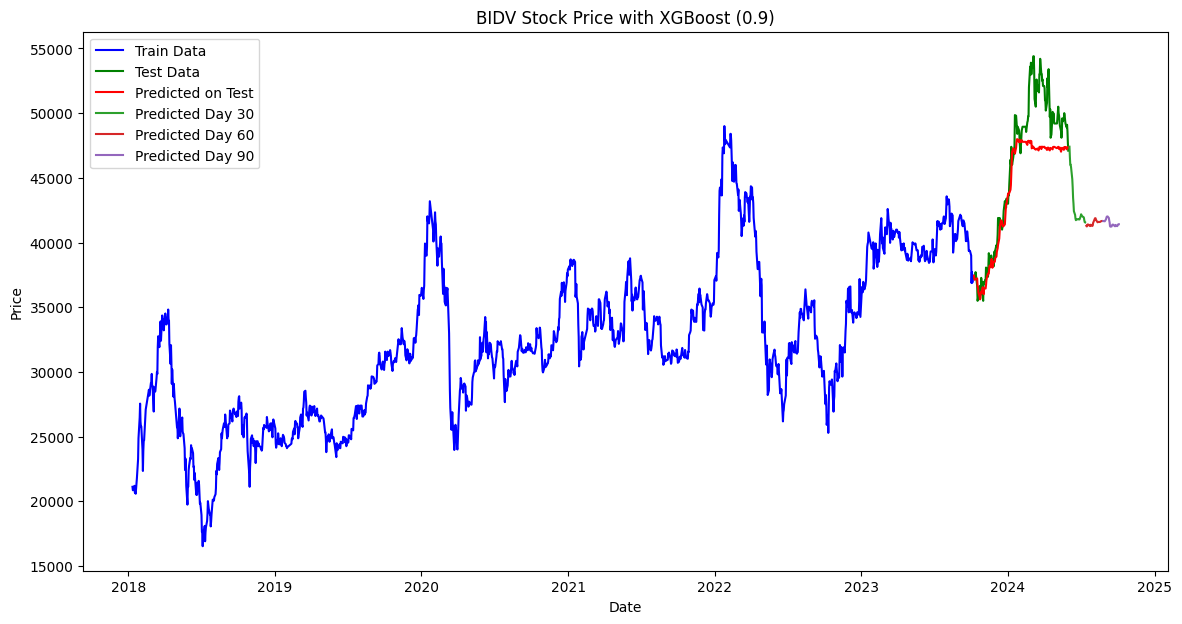
\includegraphics[width=\linewidth]{images/XGBoost/XGBoost_BIDV_91.png}
    \captionof{figure}{XGBoost with 9:1 ratio}
    \label{fig:image2}
\end{minipage}

\begin{minipage}{0.23\textwidth}
    \centering
    \includegraphics[width=\linewidth]{images}
    \captionof{figure}{Linear Regression apply CalendarFourier, DeterministicProcess with 8:2 ratio}
    \label{fig:image1}
\end{minipage}
\hfill
\begin{minipage}{0.23\textwidth}
    \centering
    \includegraphics[width=\linewidth]{images}
    \captionof{figure}{Linear Regression apply CalendarFourier, DeterministicProcess with 9:1 ratio}
    \label{fig:image2}
\end{minipage}

\begin{minipage}{0.23\textwidth}
    \centering
    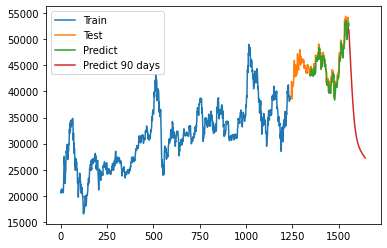
\includegraphics[width=\linewidth]{images/GRU/GRU_BIDV_90days_82.png}
    \captionof{figure}{GRU with 8:2 ratio}
    \label{fig:image1}
\end{minipage}
\hfill
\begin{minipage}{0.23\textwidth}
    \centering
    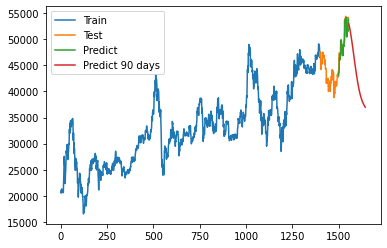
\includegraphics[width=\linewidth]{images/GRU/GRU_BIDV_90days_91.png}
    \captionof{figure}{GRU with 9:1 ratio}
    \label{fig:image2}
\end{minipage}


\begin{minipage}{0.23\textwidth}
    \centering
    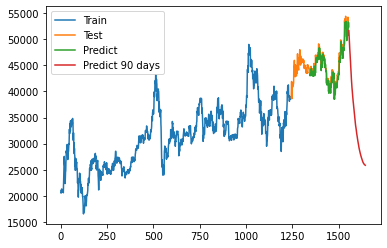
\includegraphics[width=\linewidth]{images/RNN/RNN_BIDV_90days_82.png}
    \captionof{figure}{RNN with 8:2 ratio}
    \label{fig:image1}
\end{minipage}
\hfill
\begin{minipage}{0.23\textwidth}
    \centering
    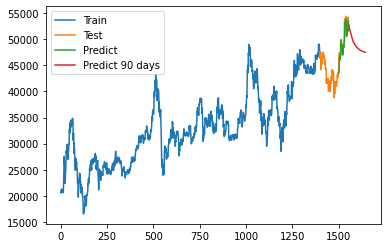
\includegraphics[width=\linewidth]{images/RNN/RNN_BIDV_90days_91.png}
    \captionof{figure}{RNN with 9:1 ratio}
    \label{fig:image2}
\end{minipage}

\begin{minipage}{0.23\textwidth}
    \centering
    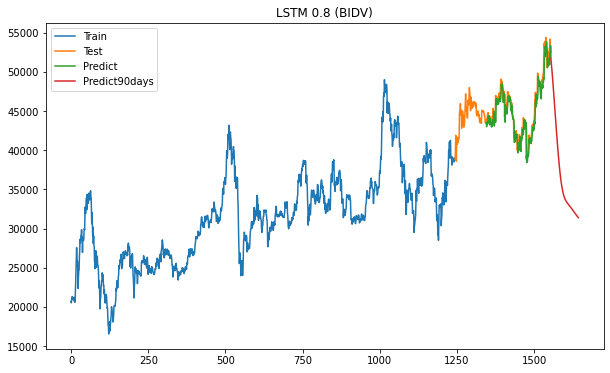
\includegraphics[width=\linewidth]{images/LSTM/LSTM_BIDV_90days_82.png}
    \captionof{figure}{LSTM with 8:2 ratio}
    \label{fig:image1}
\end{minipage}
\hfill
\begin{minipage}{0.23\textwidth}
    \centering
    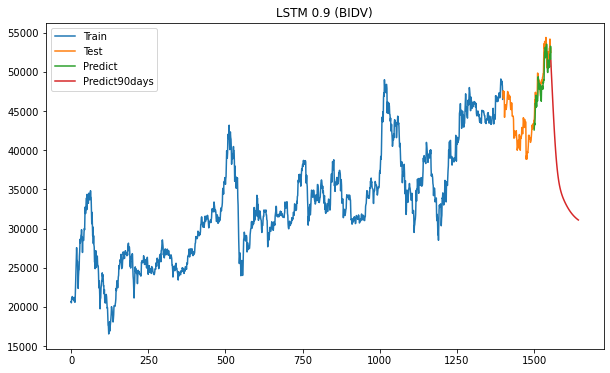
\includegraphics[width=\linewidth]{images/LSTM/LSTM_BIDV_90days_91.png}
    \captionof{figure}{LSTM with 9:1 ratio}
    \label{fig:image2}
\end{minipage}

\begin{minipage}{0.23\textwidth}
    \centering
    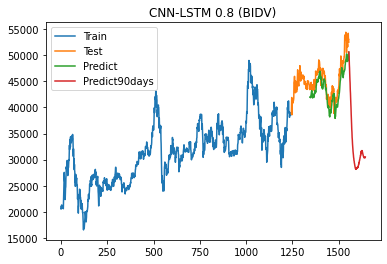
\includegraphics[width=\linewidth]{images/CNN-LSTM/CNNLSTM_BIDV_90days_82.png}
    \captionof{figure}{CNN-LSTM with 8:2 ratio}
    \label{fig:image1}
\end{minipage}
\hfill
\begin{minipage}{0.23\textwidth}
    \centering
    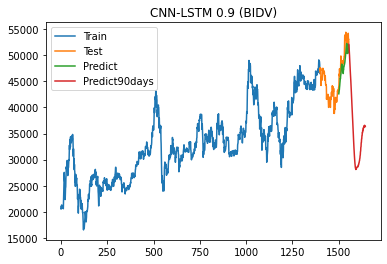
\includegraphics[width=\linewidth]{images/CNN-LSTM/CNNLSTM_BIDV_90days_91.png}
    \captionof{figure}{CNN-LSTM with 9:1 ratio}
    \label{fig:image2}
\end{minipage}

\begin{minipage}{0.23\textwidth}
    \centering
    \includegraphics[width=\linewidth]{images}
    \captionof{figure}{MICN with 8:2 ratio}
    \label{fig:image1}
\end{minipage}
\hfill
\begin{minipage}{0.23\textwidth}
    \centering
    \includegraphics[width=\linewidth]{images}
    \captionof{figure}{MICN with 9:1 ratio}
    \label{fig:image2}
\end{minipage}





\subsubsection{VCB DATASET VISUALIZATION}
\begin{minipage}{0.23\textwidth}
    \centering
    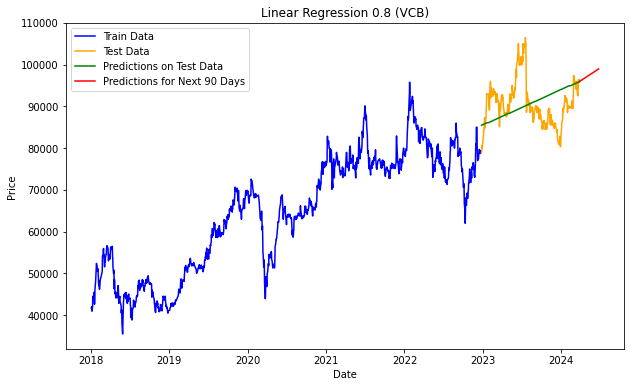
\includegraphics[width=\linewidth]{images/LR/LinearRegression_VCB_90days_82.png}
    \captionof{figure}{Linear Regression with 8:2 ratio}
    \label{fig:image1}
\end{minipage}
\hfill
\begin{minipage}{0.23\textwidth}
    \centering
    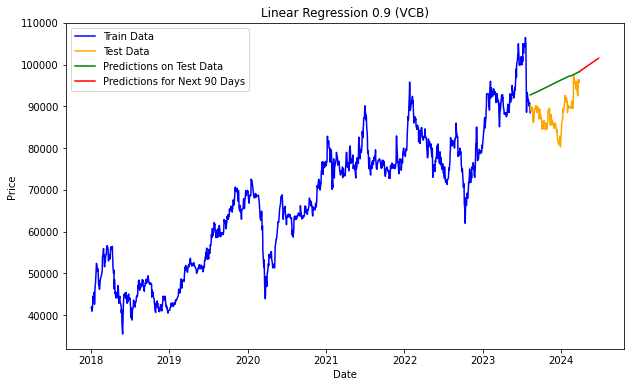
\includegraphics[width=\linewidth]{images/LR/LinearRegression_VCB_90days_91.png}
    \captionof{figure}{Linear Regression with 9:1 ratio}
    \label{fig:image2}
\end{minipage}

\begin{minipage}{0.23\textwidth}
    \centering
    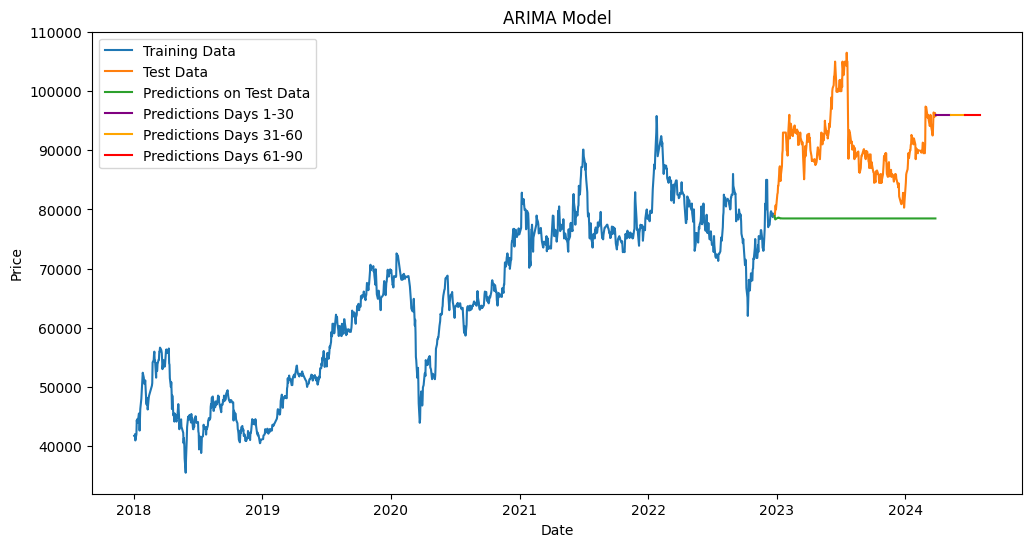
\includegraphics[width=\linewidth]{images/ARIMA/ARIMA_VCB_82.png}
    \captionof{figure}{ARIMA with 8:2 ratio}
    \label{fig:image1}
\end{minipage}
\hfill
\begin{minipage}{0.23\textwidth}
    \centering
    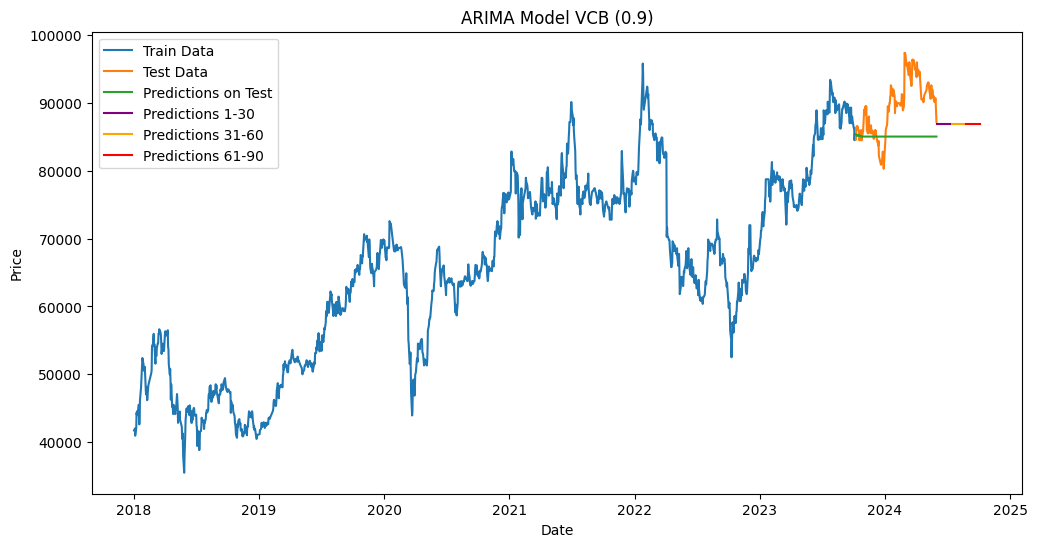
\includegraphics[width=\linewidth]{images/ARIMA/ARIMA_VCB_91.png}
    \captionof{figure}{ARIMA with 9:1 ratio}
    \label{fig:image2}
\end{minipage}

\begin{minipage}{0.23\textwidth}
    \centering
    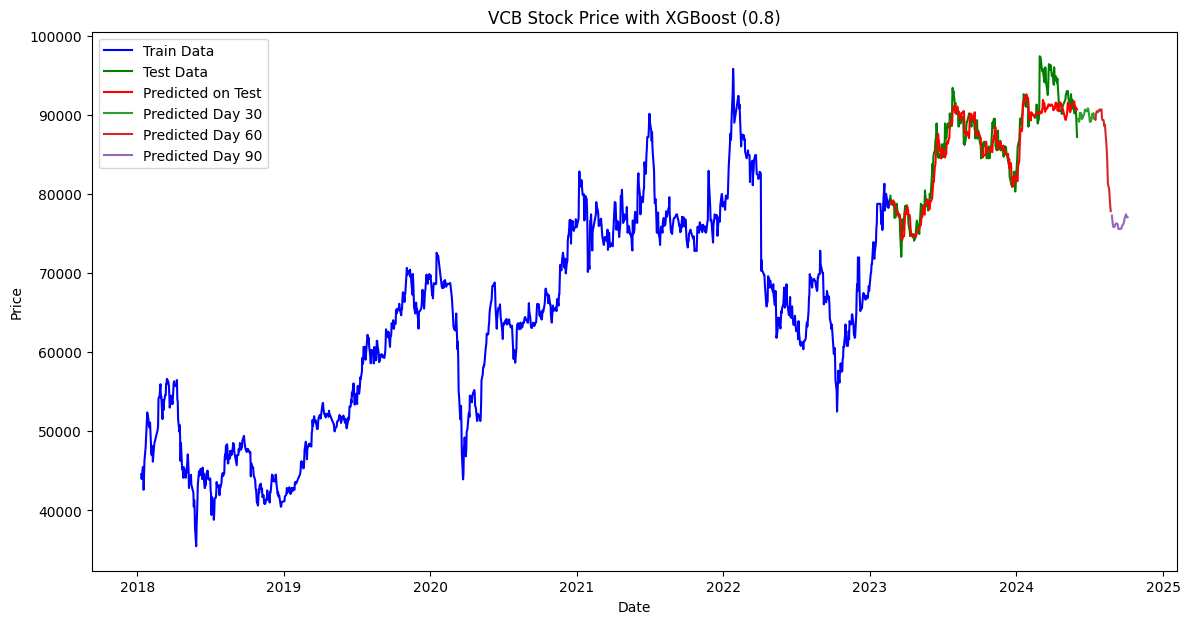
\includegraphics[width=\linewidth]{images/XGBoost/XGBoost_VCB_82.png}
    \captionof{figure}{XGBoost with 8:2 ratio}
    \label{fig:image1}
\end{minipage}
\hfill
\begin{minipage}{0.23\textwidth}
    \centering
    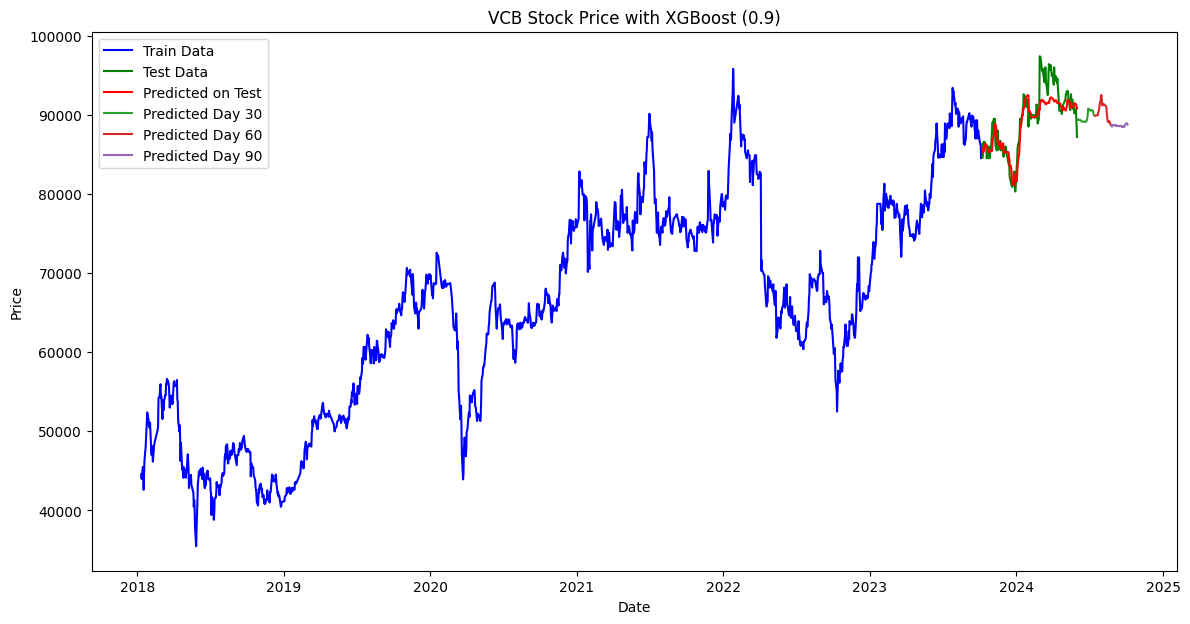
\includegraphics[width=\linewidth]{images/XGBoost/XGBoost_VCB_91.png}
    \captionof{figure}{XGBoost with 9:1 ratio}
    \label{fig:image2}
\end{minipage}

\begin{minipage}{0.23\textwidth}
    \centering
    \includegraphics[width=\linewidth]{images}
    \captionof{figure}{Linear Regression apply CalendarFourier, DeterministicProcess with 8:2 ratio}
    \label{fig:image1}
\end{minipage}
\hfill
\begin{minipage}{0.23\textwidth}
    \centering
    \includegraphics[width=\linewidth]{images}
    \captionof{figure}{Linear Regression apply CalendarFourier, DeterministicProcess with 9:1 ratio}
    \label{fig:image2}
\end{minipage}

\begin{minipage}{0.23\textwidth}
    \centering
    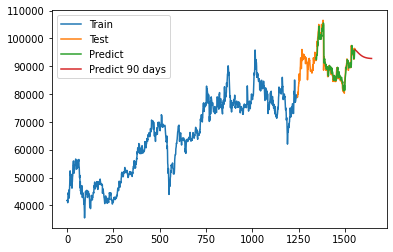
\includegraphics[width=\linewidth]{images/GRU/GRU_VCB_90days_82.png}
    \captionof{figure}{GRU with 8:2 ratio}
    \label{fig:image1}
\end{minipage}
\hfill
\begin{minipage}{0.23\textwidth}
    \centering
    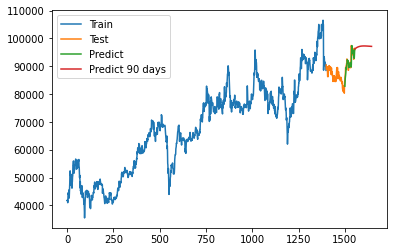
\includegraphics[width=\linewidth]{images/GRU/GRU_VCB_90days_91.png}
    \captionof{figure}{GRU with 9:1 ratio}
    \label{fig:image2}
\end{minipage}

\begin{minipage}{0.23\textwidth}
    \centering
    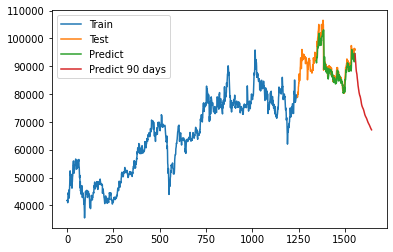
\includegraphics[width=\linewidth]{images/RNN/RNN_VCB_90days_82.png}
    \captionof{figure}{RNN with 8:2 ratio}
    \label{fig:image1}
\end{minipage}
\hfill
\begin{minipage}{0.23\textwidth}
    \centering
    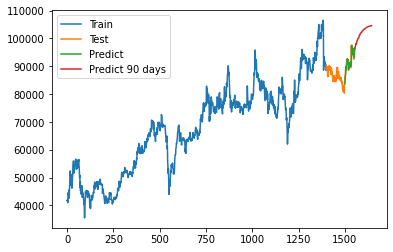
\includegraphics[width=\linewidth]{images/RNN/RNN_VCB_90days_91.png}
    \captionof{figure}{RNN with 9:1 ratio}
    \label{fig:image2}
\end{minipage}

\begin{minipage}{0.23\textwidth}
    \centering
    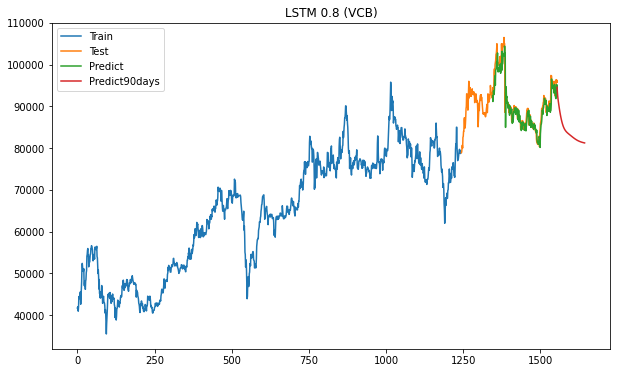
\includegraphics[width=\linewidth]{images/LSTM/LSTM_VCB_90days_82.png}
    \captionof{figure}{LSTM with 8:2 ratio}
    \label{fig:image1}
\end{minipage}
\hfill
\begin{minipage}{0.23\textwidth}
    \centering
    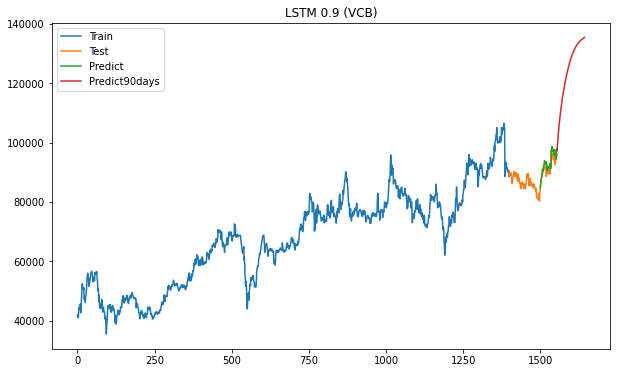
\includegraphics[width=\linewidth]{images/LSTM/LSTM_VCB_90days_91.png}
    \captionof{figure}{LSTM with 9:1 ratio}
    \label{fig:image2}
\end{minipage}

\begin{minipage}{0.23\textwidth}
    \centering
    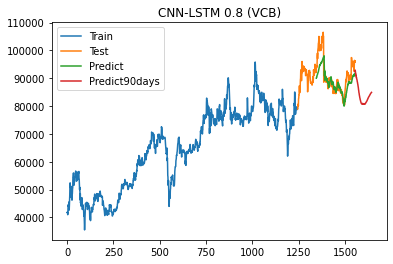
\includegraphics[width=\linewidth]{images/CNN-LSTM/CNNLSTM_VCB_90days_82.png}
    \captionof{figure}{CNN-LSTM with 8:2 ratio}
    \label{fig:image1}
\end{minipage}
\hfill
\begin{minipage}{0.23\textwidth}
    \centering
    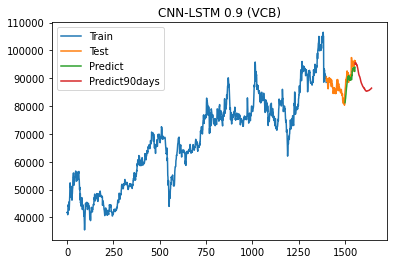
\includegraphics[width=\linewidth]{images/CNN-LSTM/CNNLSTM_VCB_90days_91.png}
    \captionof{figure}{CNN-LSTM with 9:1 ratio}
    \label{fig:image2}
\end{minipage}

\begin{minipage}{0.23\textwidth}
    \centering
    \includegraphics[width=\linewidth]{images}
    \captionof{figure}{MICN with 8:2 ratio}
    \label{fig:image1}
\end{minipage}
\hfill
\begin{minipage}{0.23\textwidth}
    \centering
    \includegraphics[width=\linewidth]{images}
    \captionof{figure}{MICN with 9:1 ratio}
    \label{fig:image2}
\end{minipage}





\subsubsection{MBB DATASET VISUALIZATION}

\begin{minipage}{0.23\textwidth}
    \centering
    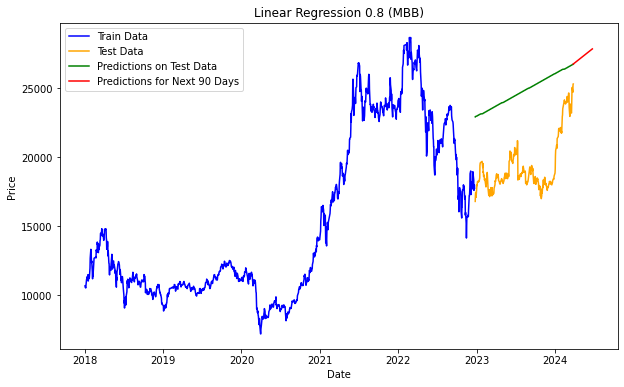
\includegraphics[width=\linewidth]{images/LR/LinearRegression_MBB_90days_82.png}
    \captionof{figure}{Linear Regression with 8:2 ratio}
    \label{fig:image1}
\end{minipage}
\hfill
\begin{minipage}{0.23\textwidth}
    \centering
    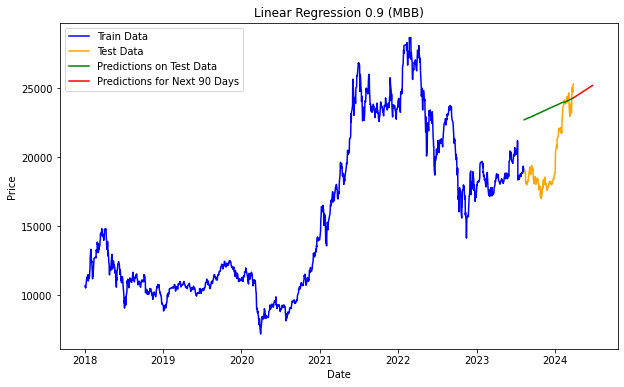
\includegraphics[width=\linewidth]{images/LR/LinearRegression_MBB_90days_91.png}
    \captionof{figure}{Linear Regression with 9:1 ratio}
    \label{fig:image2}
\end{minipage}

\begin{minipage}{0.23\textwidth}
    \centering
    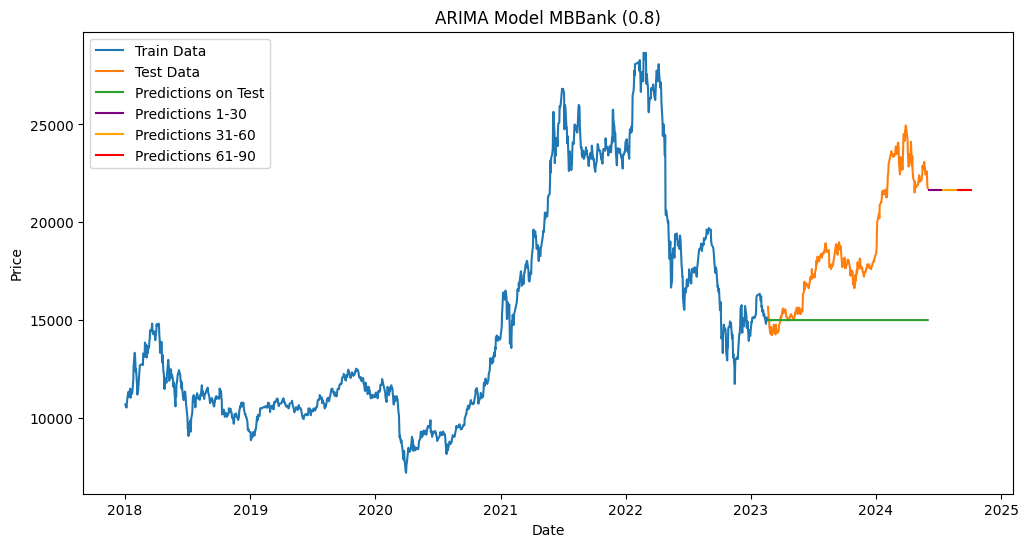
\includegraphics[width=\linewidth]{images/ARIMA/ARIMA_MBB_82.png}
    \captionof{figure}{ARIMA with 8:2 ratio}
    \label{fig:image1}
\end{minipage}
\hfill
\begin{minipage}{0.23\textwidth}
    \centering
    \includegraphics[width=\linewidth]{images/ARIMA/ARIMA_MBB_91.png}
    \captionof{figure}{ARIMA with 9:1 ratio}
    \label{fig:image2}
\end{minipage}

\begin{minipage}{0.23\textwidth}
    \centering
    \includegraphics[width=\linewidth]{images/XGBoost/XGBoost_MBB_82.png}
    \captionof{figure}{XGBoost with 8:2 ratio}
    \label{fig:image1}
\end{minipage}
\hfill
\begin{minipage}{0.23\textwidth}
    \centering
    \includegraphics[width=\linewidth]{images/XGBoost/XGBoost_MBB_91.png}
    \captionof{figure}{XGBoost with 9:1 ratio}
    \label{fig:image2}
\end{minipage}

\begin{minipage}{0.23\textwidth}
    \centering
    \includegraphics[width=\linewidth]{images}
    \captionof{figure}{Linear Regression apply CalendarFourier, DeterministicProcess with 8:2 ratio}
    \label{fig:image1}
\end{minipage}
\hfill
\begin{minipage}{0.23\textwidth}
    \centering
    \includegraphics[width=\linewidth]{images}
    \captionof{figure}{Linear Regression apply CalendarFourier, DeterministicProcess with 9:1 ratio}
    \label{fig:image2}
\end{minipage}

\begin{minipage}{0.23\textwidth}
    \centering
    \includegraphics[width=\linewidth]{images/GRU/GRU_MBB_90days_82.png}
    \captionof{figure}{GRU with 8:2 ratio}
    \label{fig:image1}
\end{minipage}
\hfill
\begin{minipage}{0.23\textwidth}
    \centering
    \includegraphics[width=\linewidth]{images/GRU/GRU_MBB_90days_91.png}
    \captionof{figure}{GRU with 9:1 ratio}
    \label{fig:image2}
\end{minipage}

\begin{minipage}{0.23\textwidth}
    \centering
    \includegraphics[width=\linewidth]{images/RNN/RNN_MBB_90days_82.png}
    \captionof{figure}{RNN with 8:2 ratio}
    \label{fig:image1}
\end{minipage}
\hfill
\begin{minipage}{0.23\textwidth}
    \centering
    \includegraphics[width=\linewidth]{images/RNN/RNN_MBB_90days_91.png}
    \captionof{figure}{RNN with 9:1 ratio}
    \label{fig:image2}
\end{minipage}

\begin{minipage}{0.23\textwidth}
    \centering
    \includegraphics[width=\linewidth]{images/LSTM/LSTM_MBB_90days_82.png}
    \captionof{figure}{LSTM with 8:2 ratio}
    \label{fig:image1}
\end{minipage}
\hfill
\begin{minipage}{0.23\textwidth}
    \centering
    \includegraphics[width=\linewidth]{images/LSTM/LSTM_MBB_90days_91.png}
    \captionof{figure}{LSTM with 9:1 ratio}
    \label{fig:image2}
\end{minipage}

\begin{minipage}{0.23\textwidth}
    \centering
    \includegraphics[width=\linewidth]{images/CNN-LSTM/CNNLSTM_MBB_90days_82.png}
    \captionof{figure}{CNN-LSTM with 8:2 ratio}
    \label{fig:image1}
\end{minipage}
\hfill
\begin{minipage}{0.23\textwidth}
    \centering
    \includegraphics[width=\linewidth]{images/CNN-LSTM/CNNLSTM_MBB_90days_91.png}
    \captionof{figure}{CNN-LSTM with 9:1 ratio}
    \label{fig:image2}
\end{minipage}

\begin{minipage}{0.23\textwidth}
    \centering
    \includegraphics[width=\linewidth]{images}
    \captionof{figure}{MICN with 8:2 ratio}
    \label{fig:image1}
\end{minipage}
\hfill
\begin{minipage}{0.23\textwidth}
    \centering
    \includegraphics[width=\linewidth]{images}
    \captionof{figure}{MICN with 9:1 ratio}
    \label{fig:image2}
\end{minipage}







\section{REFERENCE}

\printbibliography

\vspace{12pt}

\end{document}
